\subsection{Aufbau}
\label{subsec:aufbau}

Im Folgenden soll die Architektur des \gls{go1} im Detail dargestellt werden.
Hierfür werden einige Perspektiven des Roboters gezeigt, um die nach Einsatzzweck klassifizierten Bauteilgruppen zu erläutern und darzustellen.

\subsubsection{Überblick}

Die zoomorphe Form des \gls{go1} ist - wie bereits mehrfach angedeutet - an die eines Hundes angelehnt.
\todo{KAum verwendete referenz}
So ergeben sich die Bezeichnungen der äußerlich erkennbaren Bauteile von selbst.
Abbildung~\ref{fig:allgemeine_architektur} zeigt die äußerlichen Merkmale im Überblick.

\begin{figure}[h]
    \frame{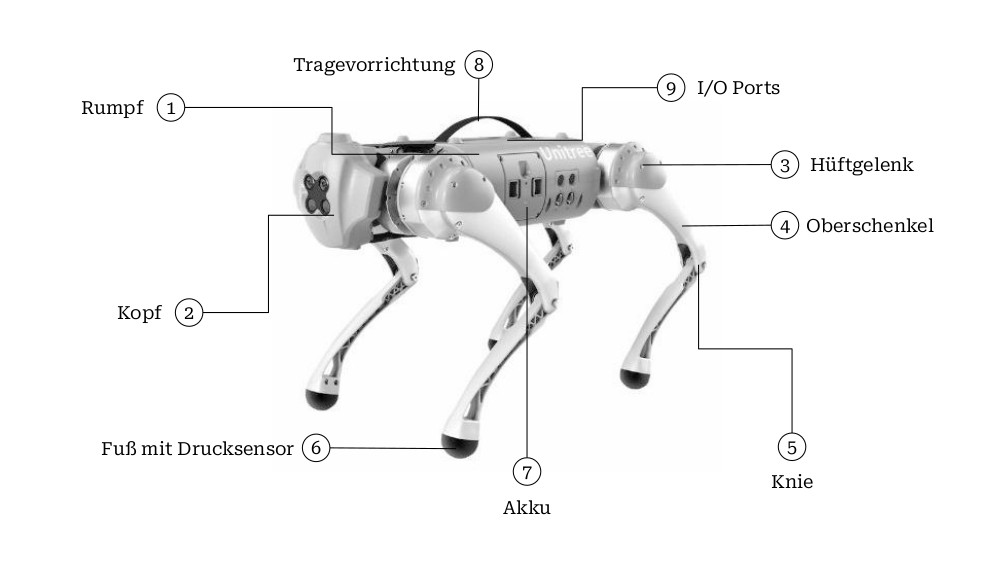
\includegraphics[width=\linewidth]{img/aufbau_intern/allgemein}}
    \caption[Überblick über den Go1]{Überblick über den GO1}\label{fig:allgemeine_architektur}
\end{figure}

Die Grundlage des Roboters bildet der Körper - auf Abbildung~\ref{fig:allgemeine_architektur} mit \numref{1} gekennzeichnet.
In diesem sind ie meisten Komponenten des \gls{go1} verbaut, unter Anderen die folgenden:
\begin{itemize}
    \item Interne Hardwarekomponenten
    \item Intelligenter Akku
    \item Teile der Sensorik und Kameras
    \item Hüftgelenke und Motoren der Beine
\end{itemize}
Eine genauere Beschreibung der Einzelteile findet sich in den folgenden Unterkapiteln.
An der Vorderseite des Körpers ist der Kopf \numref{2} des Roboters verbaut.
In diesem sind beispielsweise ein \emph{NVIDIA Jetson Xavier NX}, eine Stereo-Kamera und Stereo Ultraschall Sensoren
und weitere Bauteile wie Lautsprecher verbaut.
An den vier äußeren Ecken des Körpers sind die Beine des Roboters verbaut.
Innerhalb des Körpers sind die Motoren zur Steuerung der Hüftgelenke \numref{3} integriert.
Außerhalb der Hüftgelenke an der Oberseite der vier Oberschenkel \numref{4} sind vier weitere Motoren
zur vertikalen Steuerung der Beine verbaut.
Parallel zu diesen Motoren sind im äußeren Teil des oberen Oberschenkels identische Motoren
zur Steuerung der Knie \numref{5} integriert, die die Gelenke jeweils durch steife Achsen und Seilzüge
anwinkeln können.
An den Enden der Beine sind jeweils Füße \numref{6} verbaut, in denen Drucksensoren integriert sind.

Neben den äußerlich auffälligen Merkmalen ist auf der linken Seite des Körpers noch ein intelligenter Akku
\numref{7} verbaut.
Auf der Oberseite des Körpers sind unterhalb der Tragevorrichtung \numref{8} noch Schnittstellen \numref{9} zur physischen
Verbindung auf die integrierten Hardwarekomponenten verbaut.

% ----- Ende ----------
% ----- Überblick -----

\subsubsection{Mechanische Komponenten}

Der Anteil der in Abbildung~\ref{fig:mechanische_komponenten} gezeigten mechanischen Elemente des \gls{go1} hält sich in Grenzen.
So sind am Körper selbst lediglich vier bewegliche Teile angebaut - die vier Servomotoren
der Hüftgelenke \numref{1}.
An den Hüftgelenken befestigt sind die einzigen weiteren beweglichen Bauteile des Roboters,
die pro Bein jeweils zwei weiteren Motoren für die Neigung der Beine \numref{2} und der Kniegelenke \numref{3}.
\todo{Validieren ob starre und Seizug Verbindung genutzt werden}
\begin{figure}[h]
    \frame{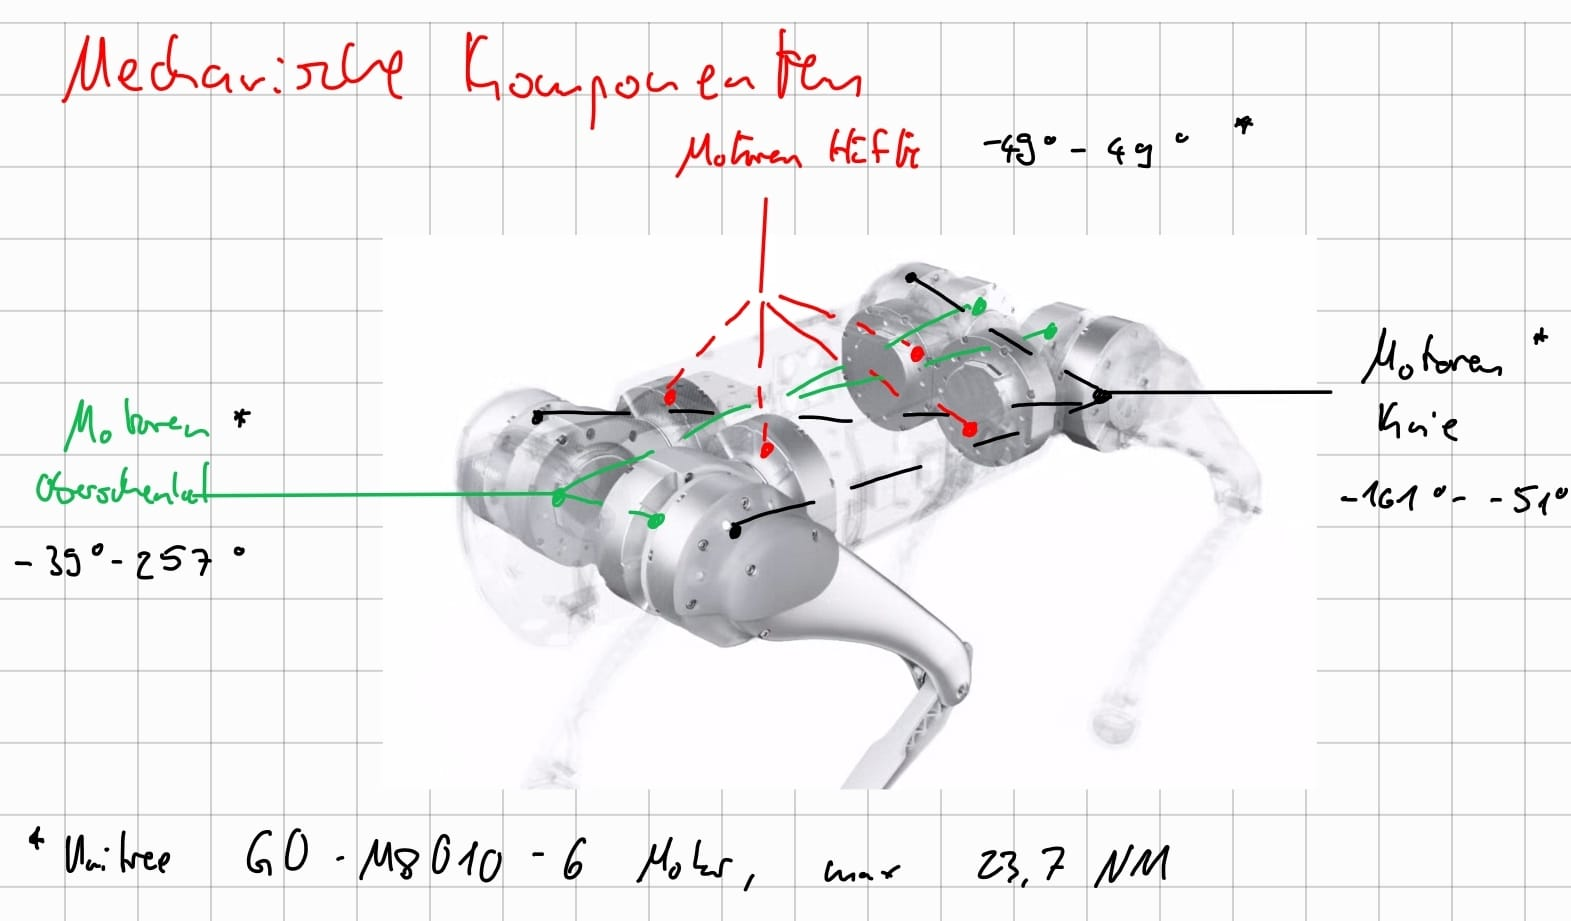
\includegraphics[width=\linewidth]{img/aufbau_intern/mechanische_komponenten}}
    \caption[Mechanische Komponenten des Go1]{Mechanische Komponenten des \gls{go1}}\label{fig:mechanische_komponenten}
\end{figure}
Zum Strecken des Kniegelenks wird eine am äußeren Motor angebrachter Seilzug \numref{4} verwendet,
zum Anwinkeln des unteren Beines wir im Gegenzug eine starre Verbindung \numref{5} an der Vorderseite des Kniegelenks genutzt.

\myparagraph{Eigenschaften der Servomotoren}
Die Servomotoren am Hüftgelenk - Abbildung~\ref{fig:mechanische_komponenten}, Bauteil \numref{1}, die Motoren an den Beininnenseiten \numref{2}
und die Motoren an den Beinaußenseiten \numref{3} sind des gleichen Models -
\emph{Unitree Robotics GO-M8010-6 Motor}\footcite{go_motor}.
Die Servomotoren \todo{Sicher Servo?} haben ein maximales Drehmoment von \num{23.7}\gls{nm} und können in 3 verschiedene Konfigurationen
eingeteilt werden:
\begin{enumerate}
    \item \textbf{Hüftmotoren}\\
    Bewegungsradius von \num{-49}\textdegree~bis \num{49}\textdegree
    \item \textbf{Oberschenkelmotoren}\\
    Bewegungsradius von \num{-39}\textdegree~bis \num{257}\textdegree
    \item \textbf{Kniemotoren}\\
    Bewegungsradius von \num{-161}\textdegree~bis \num{-51}\textdegree
\end{enumerate}
Die Motoren sind ebenfalls mit Sensorik bestückt, welche den aktuellen Zustand des Bauteils erkennen und
an die \gls{mcu} schicken können.
Diese Funktionalität wird im Kapitel~\ref{subsubsec:sensorik} näher beschrieben.

\subsubsection{Sensorik}
\label{subsubsec:sensorik}

Als wichtige Bausteine zur intelligenten Nutzung des \gls{go1} sind an vielen Stellen im Roboter
einige Sensoren oder intelligente Hardware verbaut.
Neben der dedizierten Sensorik zur Erkennung des Umfeldes ist ebenfalls einfachere Sensorik
in einigen Bauteilen wie den mechanischen Bauteilen des Laufapparats integriert.
Abbildung~\ref{fig:laufapparat} zeigt die hierfür verbauten Sensoren und intelligenten Hardwarebausteine.

\begin{figure}[h]
    \frame{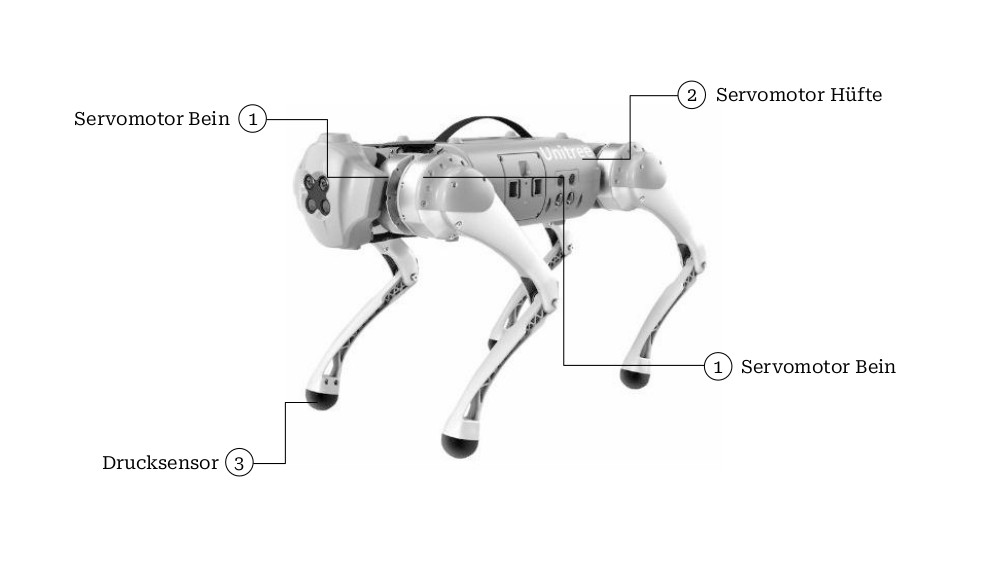
\includegraphics[width=\linewidth]{img/aufbau_intern/laufaparat}}
    \caption{Sensorik des Laufaparats}\label{fig:laufapparat}
\end{figure}

Ähnlich der mechanischen Eigenschaften der zwölf Servomotoren des Typs \emph{GO-M8010-6} - zwei pro Bein des Roboters \numref{1}
und je ein Motor im Körper des Roboters \numref{2} - sind die sensorischen Funktionen dieser identisch.
In Abbildung~\ref{fig:netzwerk_ueberblick} in Kapitel~\ref{par:netzwerk_ueberblick} ist erkennbar, dass die
zwölf Motoren des \gls{go1} über eine \emph{RS-485} Schnittstelle mit der \gls{mcu} verbunden sind.
Diese wertet die Informationen aus und steuert die einzelnen Motoren über dieselbe Schnittstelle an.
Bei Rotationsbewegungen messen die Motoren, welche Kraft für die Ausführung benötigt wird und was die Differenz zur
erwarteten Kraft ist.
So können die Motoren allein bereits eine ausreichende Datenmenge zur Steuerung des Bewegungsapparats liefern.

Als Ergänzung zur intelligenten Messung der Motoren sind in den Enden aller vier Beine \numref{3} Drucksensoren verbaut, welche
die erzeugte Kraft auf die Unterseite der Beine messen und an die \gls{mcu} senden.
Die Kombination der Rotationsdaten und -kräfte sowie der gemessenen Kräfte an den Enden der Beine ermöglichen es dem
\gls{go1}, die Motoren zum Ausgleich der Bewegungen anzusteuern und somit eine möglichst effiziente Fortbewegung zu
ermöglichen.

Neben der integrierten Sensorik zur steuerung des Laufapparats sind im \gls{go1} Kameras, Ultraschallsensoren und
Audiotechnik verbaut worden.
Abbildung \ref{fig:kameras_sensorik} zeigt hier die Verteilung der Kameras und Ultraschallsenoren.

\begin{figure}[h]
    \frame{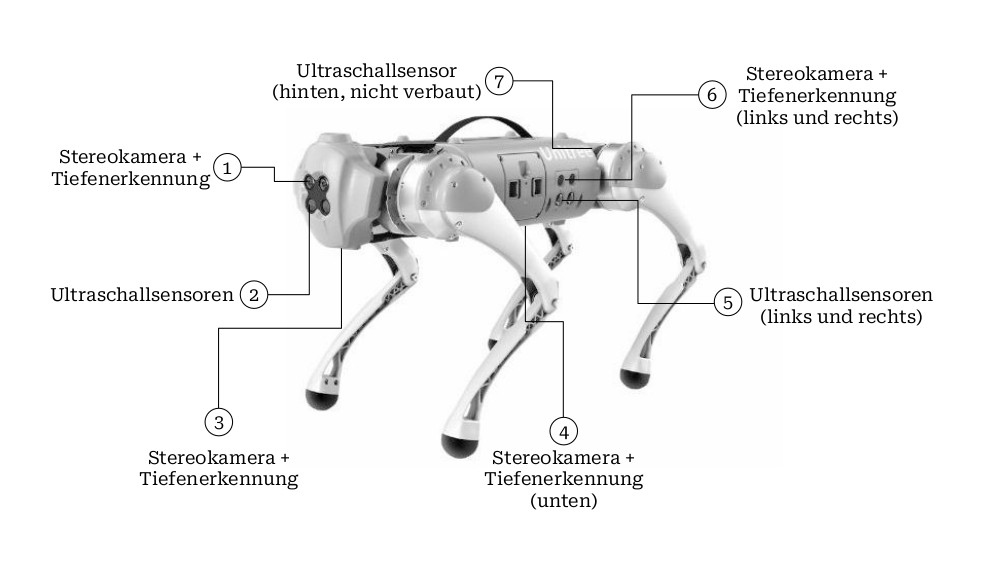
\includegraphics[width=\linewidth]{img/aufbau_intern/kameras_sensorik}}
    \caption{Darrstellung der verbauten Kamera und Sensorik}\label{fig:kameras_sensorik}
\end{figure}

Insgesamt sind im \gls{go1} fünf Stereokamerasysteme verbaut, die durch ihre doppelte Bauart ebenso zur Tiefenerkennung
fähig sind.
Die Kameras sind folgendermaßen verteilt:

\begin{itemize}
    \item \numref{1} Kopfeinheit nach vorne gerichtet
    \item \numref{3} Kopfeinheit nach unten gerichtet
    \item \numref{4} Rumpf links und rechts
    \item \numref{6} Rumpf nach unten gerichtet
\end{itemize}

Die Kameras am Kopf des \gls{go1} \numref{1} und \numref{3} werden durch den Jetson Nano im Kopf gesteuert, die beiden
nach außen gerichteten Kameras \numref{4} von einem weiteren Nano und die Kamera am Rumpf nach unten gerichtet \numref{6}
vom letzten der drei verbauten Nanos.\footcite{go1_kamera_anleitung}
Mehr zur Steuerung und den Funktionen der Kameras und Recheneinheiten in Kapitel \ref{subsec:hardware-architektur} und
\ref{subsubsec:video-streaming}.
Unter drei der fünf Kamerasysteme sind Ultraschallsensoren verbaut.
Diese sind am Kopf nach vorne gerichtet \numref{2} und am Körper zu den Seiten gerichtet \numref{5} verbaut.
Laut der Dokumentation der Ultraschallsensoren ist softwareseitig ein weiteres Ultraschallmodul am Rumpf nach hinten
gerichtet \numref{7} vorgesehen, welches aber hardwareseitig nie realisiert wurde\footcite{go1_ultraschall_anleitung}.
\todo[inline]{Prüfen, ob die seitlichen Ultraschall gekabelt und ansprechbar sind}
Die Ultraschalleinheit im Kopf des Roboters wird vom Jetson Nano im Kopf des Roboters gesteuert während die beiden seitlichen
Sensoren mit dem Raspberry Pi im Rumpf des \gls{go1} verbunden sind.


\subsubsection{Recheneinheiten und Schnittstellen}
\label{subsubsec:recheneinheiten}

Die \emph{Edu} Version des \gls{go1} ist mit einiger integrierter Rechenleistung versehen worden.
Innerhalb des Rumpfes und des Kopfes sind diverse Kleinplatinenrechner verbaut worden, um beispielsweise die Daten der oben beschriebenen
Sensoren zu verwerten, den Bewegungsapparat manuell zu manipulieren und dem Roboter weitere Funktionen hinzuzufügen.
Abbildung \ref{fig:intern} zeigt die interne Zusammensetzung des \gls{go1}.

\begin{figure}[h]
    \frame{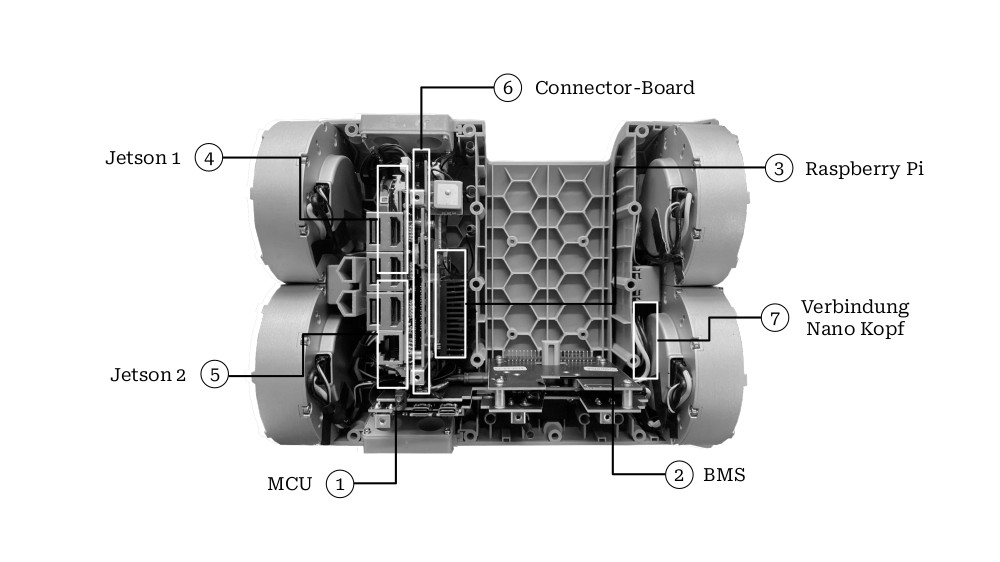
\includegraphics[width=\linewidth]{img/aufbau_intern/rechenkomponenten}}
    \caption{Blick auf die internen Komponenten}\label{fig:intern}
\end{figure}

Herzstück des Roboters ist die \gls{mcu} \numref{1}, welche auf der rechten Seite des Rumpfes verbaut ist.
Diese steuert die Motoren und greift Daten des \gls{bms} \numref{2} über den intelligenten Akku\footnote{Abbildung \ref{fig:vogelperspektive} \numref{1}}
ab.
Mittig hinter dem eingebauten Akku liegt die Kernschnittstelle des \gls{go1} mit den Nutzern, der verbaute \emph{Raspberry Pi}
\numref{3}.
Dieser ist direkt über eine Erweiterungsplatine \numref{6} für Schnittstellen und feste Verbindungen mit den beiden im Rumpf
verbauten \emph{NVIDIA Jetson Nanos} \numref{4}+\numref{5} verbunden.
Über gekabelte Verbindungen entlang des für den Akku reservierten Platzes im Rumpf verläuft die gekabelte Verbindung \numref{7}
zwischen den im Rumpf verbauten Komponenten und dem Kopf des Roboters.
Abbildung \ref{fig:kopf} zeigt die restlichen im Kopf verbauten Komponenten des Hundes.

\begin{figure}[h]
    \frame{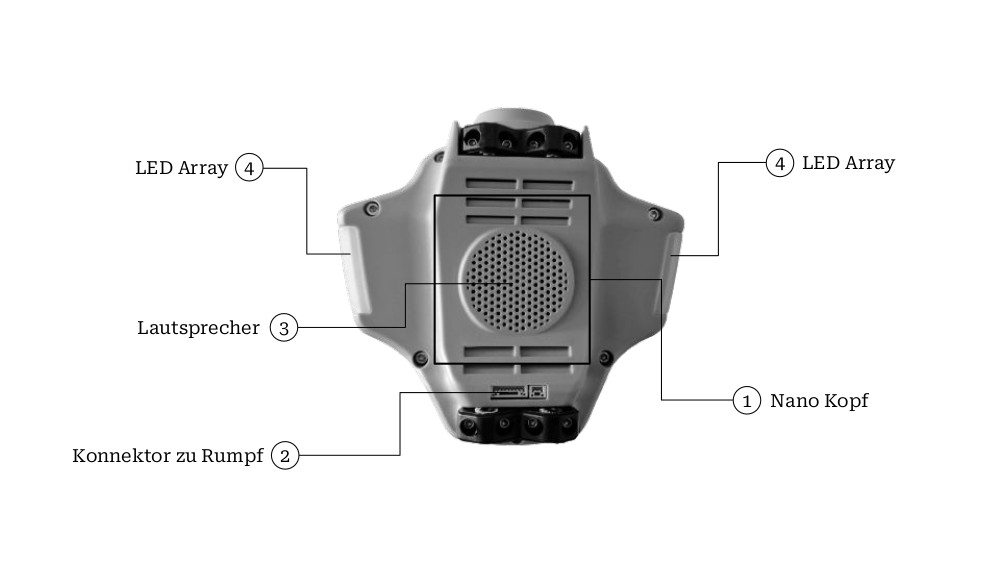
\includegraphics[width=\linewidth]{img/aufbau_intern/kopf}}
    \caption{Ansicht des Kopfes von hinten}\label{fig:kopf}
\end{figure}

Die zentrale Steuereinheit der Komponenten im Kopf des roboters ist der verbaute \emph{NVIDIA Jetson Nano} \numref{1}, der
über gekabelte Verbindungen \numref{2} mit den im Rumpf verbauten Komponenten verbunden ist.
Direkt an den Nano ist ein Lautsprecher \numref{3} verbaut, der im \emph{Edu}-Modell frei nutzbar ist\footnote{Siehe Kapitel \ref{subsubsec:audio-interfaces}}.
Ebenso direkt an den Nano angeschlossen sind links und rechts am Kopf zwei nach hinten und zur Seite orientierten
\gls{led}-Arrays.
Auch diese sind frei programmierbar\footnote{Kapitel \ref{subsubsec:led}}.
Eine detailliertere Beschreibung der Recheneinheiten und derer Funktionen folgt in Kapitel \ref{subsec:hardware-architektur}.

Auf der Oberseite des \gls{go1} sind einige Schnittstellen verbaut, die die Arbeit an den internen Komponenten und
Recheneinheiten des Roboters erleichtern sollen.
Abbildung \ref{fig:vogelperspektive} zeigt die Oberseite und die verbauten Schnittstellen.
Alternativ zur Stromversorgung über den verbauten Akku \numref{1} auf der linken Außenseite des Roboters ist eine
\emph{XT-30}-Steckverbindung \numref{2} auf der Oberseite verbaut.
Diese kann entweder den \gls{go1} anstelle des Akkus betreiben oder externe Erweiterungen durch den Akku mit Strom versorgen.
Genaueres hierzu in Kapitel \ref{subsec:inbetriebnahme}.
Direkt oberhalb dieser Verbindung sind zwei \gls{usb} \emph{Typ C} Ports \numref{3}, welche als Schnittstellen zur \gls{mcu} genutzt werden können.
Erweiterungen, wie beispielsweise \gls{gps}-Module können über eine serielle Schnittstelle \numref{4} angeschlossen werden.

\begin{figure}[h]
    \frame{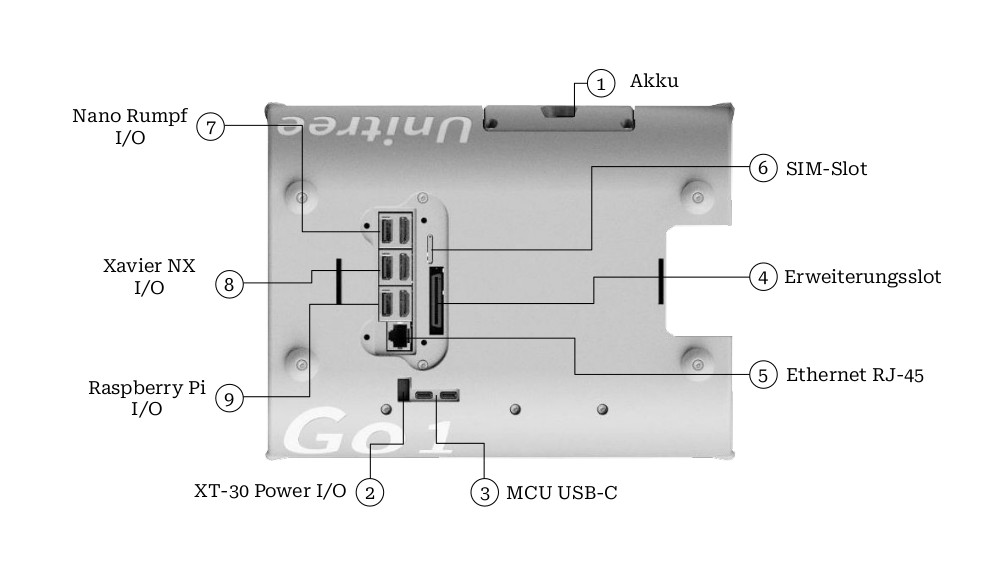
\includegraphics[width=\linewidth]{img/aufbau_intern/vogelperspektive}}
    \caption{Vogelperspektive mit Hardware}\label{fig:vogelperspektive}
\end{figure}

Zur gekabelten Verbindung eines externen Rechners mit dem intern verbauten Switch und somit den Recheneinheiten\footnote{Siehe Kapitel \ref{subsubsec:netzwerk}}
ist eine \emph{RJ-45}-Ethernetbuchse \numref{5} verbaut.
Als Alternative zum kabellosen Netzwerk kann für eine Verbindung mit dem Internet oder einem Mobilfunknetzwerk der eingebaute
Steckplatz für \emph{4G/ \gls{lte}}-Karten \numref{6} verwendet werden.
Dieser ist direkt mit dem verbauten Raspberry Pi verbunden\footnote{Siehe Kapitel \ref{subsubsec:gsm}}.

Die restlichen Verbindungen auf der Rückseite des Rumpfes sind drei Paare mit je einem \gls{hdmi} und einem \gls{usb}-A Port
Für die direkte Verbindung zu den Kleinplatinenrechnern durch Entwickler.
Die Verteilung ist wie folgt:

\begin{itemize}
    \item \numref{7} NVIDIA Jetson Nano (Rumpf)
    \item \numref{8} NVIDIA Jetson Xavier NX
    \item \numref{9} Raspberry Pi
\end{itemize}

Auf den Nano im Kopf des Roboters ist über die Ports keine direkte Verbindung möglich.




